\section{Неразмеченные данные в глубоком обучении}

\subsection{Постановка}
\hspace{2em}Общий подход к решению задачи с неразмеченными данными следующий:

$\mathcal{U} \subset \mathcal{X}$ --- большая неразмеченная выборка,

$\mathcal{D} \subset  \mathcal{X}\times \mathcal{Y}$ --- небольшая размеченная выборка,

требуется построить отображение $f: \mathcal{X} \to \mathcal{Y}$.

\subsection{Суперпозиция}
\hspace{2em}Предположение $f = c  \circ  h$ --- отображение есть суперпозия двух функций:

$h$ --- генерация признакового описания $h: \mathcal{X} \to \mathcal{H}$,

$c$ --- классификатор $c: \mathcal{H} \to \mathcal{Y}$.

Заметим, что $c$ и $h$, например, это некоторое параметрические функции, параметры которых нужно найти.

Простой пример:

$h$ --- все слои полносвязного многослойного перцептрона,

$c$ --- последний слой.

Обычно $h$ является сложной моделью, а $c$ --- линейной. Рассмотрим более подробный пример.

\subsection{Постановка задачи SimCLR}

\hspace{2em}Постановка задачи SimCLR заключается в том, что даётся набор изображений без каких-либо меток, и нужно обучить модель на этих данных так, чтобы она могла быстро адаптироваться к любой задаче распознавания изображений впоследствии.

Цель обучения - найти такое признаковое пространство, в котором изображения одного класса располагаются близко по введённой метрике, а изображения разных классов - далеко. Для этого используют различные \textit{контрастивные функции потерь}.

\begin{figure}
    \centering
    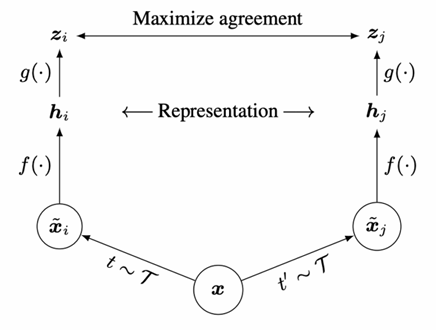
\includegraphics[width=0.5\linewidth]{chapters/unlabeled/simclr.png}
    \caption{Схематичное представление алгоритма SimCLR}
    \label{fig:enter-label-1}
\end{figure}

На рисунке можем схематичное представление последовательности шагов алгоритма со следующими обозначениями:

\begin{quote}
$x$ - исходное изображение,

$t, t'$ - разные аугментации на исходное изображение $x$ для получения представлений $\tilde{x_i}$, $\tilde{x_j}$,

$f$ - функция, генерирующая представления (representation) $h_i$, $h_j$ в виде вектора для входных изображений,

$g$ - функция, которая переводит вектора $h_i$, $h_j$ в величины $z_i$, $z_j$, для которых минимизируется расстояние (maximize agreement) в процессе обучения для аугментаций одного изображения и максимизируется для разных изображений.
\end{quote}

Шаги в обучении следующие:

1. К исходному изображению $x$ применяются аугментации $t, t'$. \textit{Аугментация} - это процесс создания новых данных на основе существующих с помощью преобразований. Такими преобразованиями для изображений являются, например, поворот, изменение яркости, гауссовское размытие и так далее. Она необходима, чтобы в новом признаковом пространстве изменённые изображения так же находились близко к изображениям того же класса.

2. К аугментированным изображениям $\tilde{x_i}$, $\tilde{x_j}$ применяется функция $f$, генерирующая векторное представление этих изображений $h_i$, $h_j$.

3. К векторным представлениям $h_i$, $h_j$ применяется функция $g$ для перевода в другое векторное представление. Данный шаг необязательный для обучения методом SimCLR.

4. Для $z_i$, $z_j$ уменьшается расстояние, если $\tilde{x_i}$, $\tilde{x_j}$ - аугментации одного и того же изображения, и увеличивается - если разных. Происходит это путём минимизации контрастивной функции потерь. 

Таким образом мы находим новое признаковое описание для изображения, с помощью которого можно обучиться на задачу классификации изображений, то есть найти функция $c$ из раздела про Суперпозицию.

\subsection{Вопросы}
\hspace{2em}1. Что такое суперпозиция в контексте построения модели для неразмеченных данных, и как она помогает в решении задачи с использованием методов глубокого обучения?

2. Каковы основные этапы и задачи в методе SimCLR?

3. Как аугментация данных способствует улучшению качества обучаемых представлений?

\section{Метод Expectation Regularization (XR)}

Рассмотрим задачу частичного обучения (\textit{semi-supervised learning}). Пусть дано множество объектов $X$ и множество классов $Y$. Предположим, что у нас имеется небольшой набор размеченных данных:
\[
X^k = \{ x_1, \ldots, x_k \} \quad \text{с метками} \quad \{y_1, \ldots, y_k\},
\]
где $y_i \in Y$ – известная метка класса для объекта $x_i$. Кроме того, нам даны неразмеченные данные:
\[
U = \{x_{k+1}, \ldots, x_{\ell}\},
\]
для которых метки классов неизвестны. Основная цель частичного обучения – используя как размеченные, так и неразмеченные данные, построить алгоритм классификации $a: X \rightarrow Y$ с лучшими обобщающими свойствами. В трансдуктивном случае, зная заранее все неразмеченные объекты, задача сводится к определению для них меток: $\{x_{k+1}, \ldots, x_{\ell}\} \rightarrow \{a_{k+1}, \ldots, a_{\ell}\}$.

Частичное обучение широко применяется: от классификации текстов и изображений до каталогизации и группировки данных в сложных приложениях, где полностью размеченные выборки собрать затруднительно или дорого.

\subsection{Многоклассовая логистическая регрессия.}

В качестве базовой модели рассмотрим многоклассовую логистическую регрессию. Предположим, что имеется конечный набор классов $Y = \{1, \ldots, |Y|\}$. Рассмотрим линейный классификатор:
\[
a(x) = \arg \max_{y \in Y} \langle w_y, x \rangle, 
\]
где $x \in \mathbb{R}^n$ – вектор признаков объекта, а $w_y \in \mathbb{R}^n$ – вектор параметров (весов) для класса $y$.

Вероятность принадлежности объекта $x_i$ классу $y$, согласно модели логистической регрессии, задаётся с помощью функции softmax:
\[
P(y \mid x_i, w) = \frac{\exp\langle w_y, x_i \rangle}{\sum_{c \in Y} \exp\langle w_c, x_i \rangle},
\]
где $w = (w_y: y \in Y)$ – совокупность всех параметров модели.

Оценка параметров модели $w$ производится путём максимизации регуляризованного правдоподобия по размеченным данным:
\[
Q(w) = \sum_{i=1}^k \log P(y_i \mid x_i, w) - \frac{1}{2C}\sum_{y \in Y}\|w_y\|^2 \;\; \to \max_w.
\]
Здесь $C > 0$ – параметр регуляризации, контролирующий степень сглаживания весов. Оптимизацию критерия $Q(w)$ обычно проводят методом стохастического градиента по параметрам $w$.

\subsection{Согласование модели на размеченных и неразмеченных данных.}

Для улучшения качества обучения в частично размеченных задачах целесообразно использовать неразмеченные данные $U = \{x_{k+1}, \ldots, x_{\ell}\}$. Пусть $b_j(x)$ – бинарный признак, связанный с объектом $x$, где $j = 1, \ldots, m$. Например, в задаче классификации текстов признак $b_j(x)$ может означать наличие или отсутствие определённого термина $j$ в документе $x$. 

Наша цель – согласовать вероятностную модель с эмпирическим распределением классов, оценённым по признакам. Рассмотрим вероятность принадлежности класса $y$ объекту, для которого признак $b_j$ активен ($b_j(x)=1$):
\[
\mathrm{P}(y \mid b_j(x)=1).
\]

Эту вероятность можно оценить двумя способами:

1. \textbf{Эмпирическая оценка} по размеченным данным $X^k$:
\[
\hat{p}_j(y) = \frac{\sum_{i=1}^k b_j(x_i)[y_i = y]}{\sum_{i=1}^k b_j(x_i)},
\]
где $[y_i = y]$ – индикаторная функция. Таким образом, $\hat{p}_j(y)$ – это частота встречаемости класса $y$ среди тех размеченных объектов, для которых признак $b_j(x)=1$.

2. \textbf{Оценка по неразмеченным данным} $U$ с использованием текущей вероятностной модели:
\[
p_j(y \mid w) = \frac{\sum_{i=k+1}^{\ell} b_j(x_i) P(y \mid x_i, w)}{\sum_{i=k+1}^{\ell} b_j(x_i)}.
\]
Здесь $P(y \mid x_i, w)$ – вероятность, предсказываемая моделью логистической регрессии, а числитель и знаменатель вычисляют взвешенную частоту класса $y$ среди объектов, в которых признак $b_j$ активен, но метки неизвестны. Таким образом, $p_j(y \mid w)$ – модельная оценка распределения классов по признаку $b_j(x)$, учитывающая неразмеченные данные.

Наша задача – приблизить модельное распределение $p_j(y \mid w)$ к эмпирическому распределению $\hat{p}_j(y)$.

\subsection{Построение регуляризатора (eXpectation Regularization, XR).}

Идея метода XR, предложенная в работе \cite{mann2007simple}, состоит в том, чтобы заставить модельные вероятности согласоваться с эмпирическими оценками. Для этого мы вводим дополнительный регуляризатор, максимизирующий логарифм правдоподобия модельных распределений с учётом признаков.

Для каждого признака $j$ рассмотрим логарифмическое правдоподобие:
\[
L_j(w) = \sum_{y \in Y} \hat{p}_j(y) \log p_j(y \mid w).
\]
Максимизация $L_j(w)$ по $w$ стремится сделать модельные оценки распределения классов по признаку $b_j$ максимально близкими к эмпирическим оценкам. 

Объединяя это с исходным критерием $Q(w)$, получаем:
\[
Q(w) + \gamma \sum_{j=1}^m L_j(w) = \sum_{i=1}^k \log P(y_i \mid x_i, w) 
- \frac{1}{2C}\sum_{y \in Y}\|w_y\|^2 +
\]
\[
+ \gamma \sum_{j=1}^m \sum_{y \in Y} \hat{p}_j(y)\log\left(\sum_{i=k+1}^{\ell} b_j(x_i)P(y \mid x_i, w)\right) \;\; \to \max_w.
\]

Здесь $\gamma > 0$ – коэффициент, отвечающий за степень влияния регуляризации XR. Итоговый критерий учитывает как размеченные данные (первое слагаемое), так и неразмеченные данные через эмпирические распределения по признакам (слагаемое с $L_j(w)$).

Оптимизация проводится методом стохастического градиента, обновляя параметры $w$ итеративно.

\subsection{Особенности и преимущества метода XR.}

Метод XR обладает рядом преимуществ и особенностей:

1. XR – это метод частичного обучения, но он \textbf{не} основан на кластеризации. Вместо этого он стремится согласовать распределения классов, предсказываемые моделью, с эмпирическими распределениями по признакам, оцененными по ограниченному набору размеченных данных.

2. Оптимизация осуществляется методом стохастического градиента, что обеспечивает масштабируемость на большие объемы данных.

3. Выбор признаков $b_j(x)$:

--- Если $b_j(x) \equiv 1$ для всех $x$, тогда $p_j(y \mid b_j(x)=1)$ интерпретируется как априорная вероятность класса $y$. Данная модель называется \textit{label regularization}, она особенно полезна в задачах с несбалансированными классами.

--- Если $b_j(x)$ указывает на присутствие или отсутствие конкретного термина $j$ в тексте $x$, то он подходит для классификации текстовых данных, так как учитывает распределение классов по характерным признакам.

4. Метод XR слабо чувствителен к выбору гиперпараметров $C$ и $\gamma$, устойчив к погрешностям в оценках $\hat{p}_j(y)$ и не требует большого числа размеченных объектов $k$.

5. XR хорошо работает в задачах категоризации текстов, где есть много неразмеченных данных, а получение полного набора разметки обходится слишком дорого или занимает много времени.

\subsection{Задачи.}

\bigskip

\noindent\textbf{Задача 1. Вычисление градиента XR-члена функционала}

Рассмотрим XR-член функционала:
\[
F_{\text{XR}}(w) = \gamma \sum_{j=1}^m \sum_{y \in Y} \hat{p}_j(y) \log\left(\sum_{x \in U_j} P(y \mid x,w)\right),
\]
где $U_j = \{ x_{k+1}, \ldots, x_{\ell} \mid b_j(x)=1 \}$ — подмножество неразмеченных объектов, для которых признак $b_j$ активен, и $\hat{p}_j(y)$ — эмпирическое распределение классов по признаку $b_j$.

Найдите градиент $F_{\text{XR}}(w)$ по параметрам $w_y$.

\subsubsection*{Решение:}

Обозначим
\[
A_{j,y}(w) = \sum_{x \in U_j} P(y \mid x,w).
\]

Тогда
\[
F_{\text{XR}}(w) = \gamma \sum_{j=1}^m \sum_{y \in Y} \hat{p}_j(y) \log A_{j,y}(w).
\]

Частная производная по $w_y$:
\[
\nabla_{w_y} F_{\text{XR}}(w) = \gamma \sum_{j=1}^m \sum_{y' \in Y} \hat{p}_j(y') \frac{1}{A_{j,y'}(w)} \sum_{x \in U_j} \nabla_{w_y}P(y' \mid x,w).
\]

Для логистической регрессии:
\[
\nabla_{w_y}P(y' \mid x,w) = P(y' \mid x,w)(\mathbb{I}[y'=y]-P(y \mid x,w))x.
\]

Подставляя в выражение:
\[
\nabla_{w_y} F_{\text{XR}}(w) = \gamma \sum_{j=1}^m \sum_{y' \in Y} \hat{p}_j(y') \frac{\sum_{x \in U_j} P(y' \mid x,w)(\mathbb{I}[y'=y]-P(y \mid x,w))x}{A_{j,y'}(w)}.
\]

Таким образом, мы получили формулу для градиента по параметрам $w_y$ от XR-члена функционала.

\bigskip

\noindent\textbf{Задача 2. Смешанное влияние априорных предположений и неразмеченных данных}

Пусть мы имеем априорное предположение о распределении классов (например, мы знаем, что класс $y=1$ встречается в 70\% случаев), а также большие неразмеченные данные $U$. Объясните, как совместный учёт априорной информации и структуры неразмеченного множества может улучшить точность классификации по сравнению с использованием только одного из этих источников информации.

\subsubsection*{Решение:}
Априорное предположение о распределении классов помогает задать общий «баланс» между классами и избежать смещения в пользу редких классов. Однако без знания структуры данных оно может быть неточно применено. Неразмеченные данные дают понимание структуры распределения: где классы могут располагаться и как данные группируются. Совместное использование: априорная вероятность подсказывает, какие классы более вероятны в целом, а структура $U$ уточняет, где должна проходить граница, чтобы согласовать эти вероятности с реальным расположением точек. В итоге мы получаем более точный классификатор, чем если бы полагались исключительно на априор или только на структуру $U$.

\bigskip

\noindent\textbf{Задача 3. Интерпретация XR через эмпирические распределения}

Пусть у нас есть многоклассовая логистическая регрессия с параметрами $w$ и небольшой набор размеченных данных $X^k$. Для каждого бинарного признака $b_j(x)$ по размеченной части мы можем оценить эмпирическое распределение классов $\hat{p}_j(y)$. Метод XR добавляет к исходному критерию $Q(w)$ дополнительное слагаемое:
\[
\gamma \sum_{j=1}^m \sum_{y \in Y} \hat{p}_j(y) \log p_j(y \mid w),
\]

Объясните, почему максимизация совокупной функции стремится «подтянуть» модельные вероятности $p_j(y \mid w)$ к эмпирическим оценкам $\hat{p}_j(y)$. В чём заключается смысл регуляризатора XR с точки зрения использования информации о неразмеченных данных?

\subsubsection*{Решение:} 
Регуляризатор стремится сделать так, чтобы предсказания по неразмеченным данным были согласованы с эмпирическими частотами классов по признакам, оцененными на размеченных данных. Это означает, что модель не просто настраивается по размеченным объектам напрямую, но и пытается воспроизводить выявленные «шаблоны» вероятностей классов, используя набор неразмеченных объектов для уточнения вероятностных оценок. 

С точки зрения дивергенции Кульбака-Лейблера (KL-дивергенции), это дополнение минимизирует расхождение между эмпирическими распределениями $\hat{p}_j(y)$ и модельными предсказаниями $p_j(y \mid w)$. KL-дивергенция измеряет, насколько распределение $p_j(y \mid w)$ плохо аппроксимирует эмпирическое распределение $\hat{p}_j(y)$, и штрафует модель за это несоответствие. Таким образом, минимизация KL-дивергенции приводит к «подтягиванию» вероятностей модели к эмпирическим данным.

Смысл регуляризатора XR заключается в том, чтобы использовать информацию о неразмеченных данных для уточнения вероятностных оценок, согласованных с эмпирическими закономерностями, обнаруженными в размеченной выборке. Это снижает риск переобучения, улучшает обобщающую способность модели и позволяет использовать априорные знания для улучшения её предсказаний.

